\documentclass[12pt]{article}

\usepackage[margin = 1in]{geometry}
\usepackage{amsmath}
\usepackage{amssymb}
\usepackage{bm}
\usepackage{tikz}
\usepackage{mathtools}
\usetikzlibrary{automata,positioning,arrows.meta,calc}
\tikzset{>={Latex[scale=1.5]}}

\begin{document}

\title{CS 3133: Homework 4}
\author{Adam Camilli (aocamilli@wpi.edu)}
\date{\today}
\maketitle

\begin{enumerate}
\item Use the technique from Section 6.1 in the book to build the
  state diagram of an NFA-$\lambda$ that accepts the language
  $\bm{b(ab)^{\star}b}$. \\ \\
  To build this language using the recursive definition of regular
  languages in the manner described in Section 6.1, we can build
  the language $b(ab)^{\star}b$ using the singleton sets $\{a\} \text{ and } \{b\}$. The
  only tricky part is that we are not interested in only $\{ab\}$ but
  $\{ab\}^{\star}$. This is easily represented, however, with a
  looping $\lambda$-transition:

  \begin{center}
    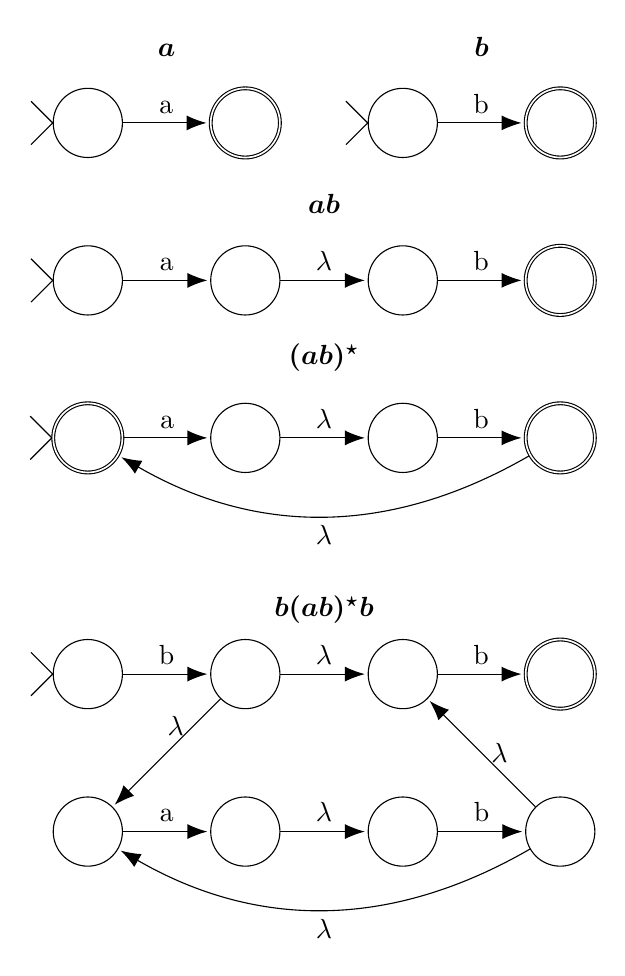
\begin{tikzpicture}[shorten >=1pt, node distance=2cm, auto]

      \node[state] (q0a) {}; %starting node
      \draw (q0a.west) -- ++(-3mm,3mm);
      \draw (q0a.west) -- ++(-3mm,-3mm);
      \node[label={$\bm{a}$}] (q0a_title) at (1, 0.6) {};
      \node[state,accepting] (q1a) [right of=q0a] {};
      \node[state] (q0b) [right of=q1a] {}; %starting node
      \draw (q0b.west) -- ++(-3mm,3mm);
      \draw (q0b.west) -- ++(-3mm,-3mm);
      \node[label={$\bm{b}$}] (q0b_title) at (1+2+1+1,0.6) {};
      \node[state,accepting] (q1b) [right of=q0b] {};
      \node[state] (q0ab) [below of=q0a] {}; %starting node
      \draw (q0ab.west) -- ++(-3mm,3mm);
      \draw (q0ab.west) -- ++(-3mm,-3mm);
      \node[label={$\bm{ab}$}] (q0ab_title) at (1+2, 0.6-2) {};
      \node[state] (q1ab) [right of=q0ab] {};
      \node[state] (q2ab) [right of=q1ab] {};
      \node[state,accepting] (q3ab) [right of=q2ab] {};
      \node[state,accepting] (q0ab*) [below of=q0ab] {}; %starting node
      \draw (q0ab*.west) -- ++(-3mm,3mm);
      \draw (q0ab*.west) -- ++(-3mm,-3mm);
      \node[label={$\bm{(ab)^{\star}}$}] (q0ab*_title) at (1+2, 0.6-2-2) {};
      \node[state] (q1ab*) [right of=q0ab*] {};
      \node[state] (q2ab*) [right of=q1ab*] {};
      \node[state,accepting] (q3ab*) [right of=q2ab*] {};
      \node[state] (q0full) at (0,-7) {}; %starting node
      \draw (q0full.west) -- ++(-3mm,3mm);
      \draw (q0full.west) -- ++(-3mm,-3mm);
      \node[label={$\bm{b(ab)^{\star}b}$}] (q0full_title) at (1+2, 0.6-7-0.2) {};
      \node[state] (q1full) [right of=q0full] {};
      \node[state] (q2full) [below of=q0full] {};
      \node[state] (q3full) [right of=q2full] {};
      \node[state] (q4full) [right of=q3full] {};
      \node[state] (q5full) [right of=q4full] {};
      \node[state] (q6full) [right of=q1full] {};
      \node[state,accepting] (q7full) [right of=q6full] {};
      
      \path[->] (q0a) edge node {a} (q1a)
                (q0b) edge node {b} (q1b)
                (q0ab) edge node {a} (q1ab)
                (q1ab) edge node {$\lambda$} (q2ab) 
                (q2ab) edge node {b} (q3ab)
                (q0ab*) edge node {a} (q1ab*)
                (q1ab*) edge node {$\lambda$} (q2ab*)
                (q2ab*) edge node {b} (q3ab*)
                (q3ab*) edge [bend left] node {$\lambda$} (q0ab*)

                (q0full) edge node {b} (q1full)
                (q1full) edge node {$\lambda$} (q6full)
                (q1full) edge [left, near start] node {$\lambda$} (q2full)
                (q2full) edge node {a} (q3full)
                (q3full) edge node {$\lambda$} (q4full)
                (q4full) edge node {b} (q5full)
                (q5full) edge [bend left] node {$\lambda$} (q2full)
                (q5full) edge [right, midway] node {$\lambda$} (q6full)
                (q6full) edge node {b} (q7full);
                
              \end{tikzpicture}
            \end{center}
\newpage
  
\item \textbf{6.3} (p. 217) The language of the DFA M in Example 5.3.7
  consists of all strings over $\{a,b\}$ with an even number of $a$'s
  and an odd number of $b$'s. Use Algorithm 6.2.2 to construct a
  regular expression L(M). Exercise 2.38 requested a nonalgorithmic
  construction of a regular expression for this language, which, as
  you now see, is a formidable task. \\ \\

  M:
  \begin{center}
    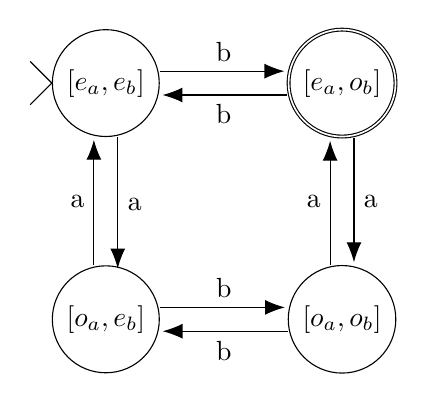
\begin{tikzpicture}[shorten >= 1pt, node distance = 3cm, auto]
      \node[state] (q0) {$[e_a,e_b]$};  %starting node
      \draw (q0.west) -- ++(-3mm,3mm);
      \draw (q0.west) -- ++(-3mm,-3mm);
      \node[state] (q1) [below of=q0] {$[o_a,e_b]$};
      \node[state] (q2) [right of=q1] {$[o_a,o_b]$};
      \node[state,accepting] (q3) [right of=q0] {$[e_a,o_b]$};
 
      \path[->] ([xshift=1ex]q0.south) edge node {a} ([xshift=1ex,yshift=-0.5ex]q1.north)
                ([yshift=1ex]q0.east) edge node {b} ([yshift=1ex]q3.west)
                ([xshift=-1ex]q1.north) edge node {a} ([xshift=-1ex]q0.south)
                ([yshift=1ex]q1.east) edge node {b} ([yshift=1ex]q2.west)
                ([yshift=-1ex]q2.west) edge node {b} ([yshift=-1ex]q1.east)
                ([xshift=-1ex]q2.north) edge node {a} ([xshift=-1ex]q3.south)
                ([xshift=1ex]q3.south) edge node {a} ([xshift=1ex]q2.north)
                ([yshift=-1ex]q3.west) edge node {b} ([yshift=-1ex]q0.east);
              \end{tikzpicture}
            \end{center}

     We begin by deleting state $[o_a, e_b]$, or $q_1$. Following the
     algorithm, we obtain the following replacement transitions:
     \begin{center}
       \begin{tabular}{c|c}
         $q_0\rightarrow q_1 \rightarrow q_2$ & $q_0 \xrightarrow{ab} q_2$ \\
         \hline
         $q_2\rightarrow q_1 \rightarrow q_0$ & $q_2 \xrightarrow{ba} q_0$ \\
         \hline
         $q_0\rightarrow q_1 \rightarrow q_0$ & $q_0 \xrightarrow{aa} q_0$ \\
         \hline
         $q_2\rightarrow q_1 \rightarrow q_2$ & $q_2 \xrightarrow{bb} q_2$ \\
       \end{tabular}
     \end{center}

     This gives the following DFA:
     \begin{center}
       \begin{tikzpicture}[shorten >= 1pt, node distance = 3cm, auto]
         \node[state] (q0) {$[e_a,e_b]$};  %starting node
         \draw (q0.west) -- ++(-3mm,3mm);
         \draw (q0.west) -- ++(-3mm,-3mm);
         \node[state] (q2) [below of=q3] {$[o_a,o_b]$};
         \node[state,accepting] (q3) [right of=q0] {$[e_a,o_b]$};
         
         \path[->] 
         ([yshift=1ex]q0.east) edge node {b} ([yshift=1ex]q3.west)
         (q0) edge node {ab} (q2)
         (q2) edge [bend left] node {ba} (q0)
         ([xshift=-1ex]q2.north) edge node {a} ([xshift=-1ex]q3.south)
         ([xshift=1ex]q3.south) edge node {a} ([xshift=1ex]q2.north)
         ([yshift=-1ex]q3.west) edge node {b} ([yshift=-1ex]q0.east);
       \end{tikzpicture}
     \end{center}

\newpage

     Now delete state $[o_a,o_b]$, or $q_2$:

     \begin{center}
       \begin{tabular}{c|c}
         $q_0\rightarrow q_1 \rightarrow q_2$ & $q_0 \xrightarrow{ab(bb)^{\star}a
                                                \cup b} q_2$ \\
         \hline
         $q_2\rightarrow q_1 \rightarrow q_0$ & $q_2 \xrightarrow{a(bb)^{\star}ba
                                                \cup b} q_0$ \\
         \hline
         $q_0\rightarrow q_1 \rightarrow q_0$ & $q_0
                                                \xrightarrow{ab(bb)^{\star}ba
                                                \cup aa} q_0$ \\
         \hline
         $q_2\rightarrow q_1 \rightarrow q_2$ & $q_2 \xrightarrow{a(bb)^{\star}a}q_2$ \\
       \end{tabular}
     \end{center}
     
     which gives the two state DFA
     \begin{center}
       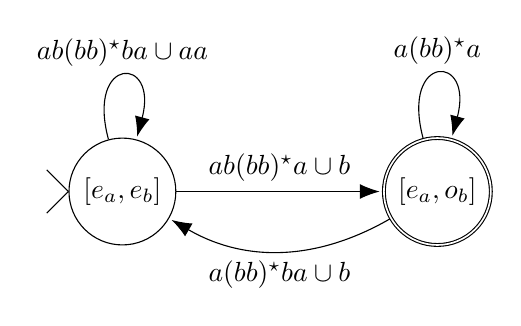
\begin{tikzpicture}[shorten >= 1pt, node distance = 4cm, auto]
         \node[state] (q0) {$[e_a,e_b]$};  %starting node
         \draw (q0.west) -- ++(-3mm,3mm);
         \draw (q0.west) -- ++(-3mm,-3mm);
         \node[state,accepting] (q3) [right of=q0] {$[e_a,o_b]$};
         
         \path[->] 
         (q0) edge [loop above] node {$ab(bb)^{\star}ba \cup aa$} (q3)
         (q0) edge node {$ab(bb)^{\star}a \cup b$} (q3)
         (q3) edge [bend left] node {$a(bb)^{\star}ba \cup b$} (q0)
         (q3) edge [loop above] node {$a(bb)^{\star}a$} (q3);
       \end{tikzpicture}
     \end{center}
     
     and at last allows us to construct an expression L(M) which
     accepts the language using the rule for a two-state DFA where
     $q_0 \neq q_f$. 
     \begin{align*}
       u &= ab(bb)^{\star}ba \cup aa \\
       v &= ab(bb)^{\star}a \cup b \\
       w &= a(bb)^{\star}a \\
       x &= a(bb)^{\star}ba \cup b 
     \end{align*}
     \[\text{L(M) } = u^{\star}v\big(w \cup xu^{\star}v^{\star}\big)^{\star}\]
  

\newpage

\item \textbf{6.4} (p. 217) Let G be the grammar
  \begin{align*}
    G: S \rightarrow \text{ }& aS\text{ $\vert$ }bA\text{ $\vert$ }a \\
    A \rightarrow \text{ }& aS\text{ $\vert$ }bA\text{ $\vert$ }b. \\
  \end{align*}
  \begin{enumerate}
  \item Use Theorem 6.3.1 to build an NFA M that accepts L(G). \\ \\
    Per the theorem, we define our new NFA-$\lambda$ as having states
    $Q$ such that
    \[ Q = \{S,A,Z\} \]
    where $Z$ contains all terminal productions, which here are 
    \[S \rightarrow a \]
    \[A \rightarrow b \]
    We now replace all productions of the form $A \rightarrow aB$ with
    a transition $\delta(A,a)=B$:
    \begin{align*}
      S \rightarrow aS &\Rightarrow \delta(S,a) = S \\
      S \rightarrow bA &\Rightarrow \delta(S,b) = A \\
      A \rightarrow aB &\Rightarrow \delta(A,a) = S \\
      A \rightarrow bA &\Rightarrow \delta(A,b) = A 
    \end{align*}
    Finally, we can construct the NFA with states $S, A, Z$ where $Z$
    is our accepting state:
    
    \begin{center}
      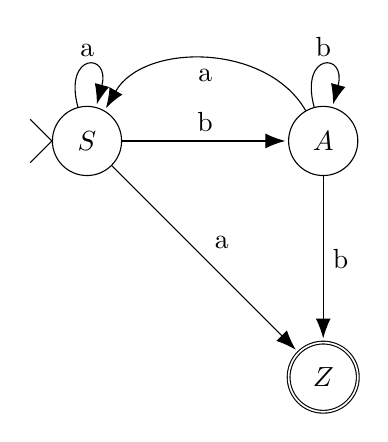
\begin{tikzpicture}[shorten >= 1pt, node distance = 3cm, auto]
        \node[state] (S) {$S$};  %starting node
        \draw (S.west) -- ++(-3mm,3mm);
        \draw (S.west) -- ++(-3mm,-3mm);
        \node[state] (A) [right of=S] {$A$};
        \node[state,accepting] (Z) [below of=A] {$Z$};
        
        \path[->] 
        (S) edge [loop above] node {a} (S)
        (S) edge node {b} (A)
        (S) edge node {a} (Z)
        (A) edge [loop above] node {b} (A)
        (A) edge [bend right=60] node {a} (S)
        (A) edge node {b} (Z);
      \end{tikzpicture}
    \end{center}
     
\newpage
    
  \item Using the result of part (a), build a DFA M$'$ that accepts
    L(G).
    Using $q_0 = S, q_1 = \{S,Z\}, q_2 = A, q_3 = \{A,Z\}$ :
    \begin{center}
      \begin{tabular}{c|cc}
        & a & b \\
        \hline
        $q_0$ & $q_1$ & $q_2$ \\
        $q_1$ & $q_1$ & $q_2$ \\ 
        $q_2$ & $q_0$ & $q_3$ \\
        $q_3$ & $q_0$ & $q_3$ \\
      \end{tabular}
    \end{center}
    
    \begin{center}
      \begin{tikzpicture}[shorten >= 1pt, node distance = 3cm, auto]
        \node[state] (q0) {$q_0$};  %starting node
        \draw (S.west) -- ++(-3mm,3mm);
        \draw (S.west) -- ++(-3mm,-3mm);
        \node[state,accepting] (q1) [right of=q0] {$q_1$};
        \node[state] (q2) [below of=q1] {$q_2$};
        \node[state,accepting] (q3) [left of=q2] {$q_3$};
        
        \path[->] 
        (q0) edge node {a} (q1)
        (q0) edge [bend right] node {b} (q2)
        (q1) edge [loop above] node {a} (q1)
        (q1) edge node {b} (q2)
        (q2) edge [bend right] node {a} (q0)
        (q2) edge node {b} (q3)
        (q3) edge [loop below] node {b} (q3)
        (q3) edge node {a} (q0);
      \end{tikzpicture}
    \end{center}
        

  \item Construct a regular grammar from M that generates L(M). 
    \begin{align*}
      S &\rightarrow aS|aZ|bA \\
      A &\rightarrow bA|bZ|aS \\
      Z &\rightarrow \lambda 
    \end{align*}
  \item Construct a regular grammar from M$'$ that generates L(M$'$).
    \begin{align*}
      S &\rightarrow aA|a \\
      A &\rightarrow aA|bB|a \\
      B &\rightarrow aS|bZ|b \\
      Z &\rightarrow bZ|aS|b 
    \end{align*}
  \item Give a regular expression for L(G).
    \[(a^{\star}bb^{\star}a)^{\star}a^+
      \cup (a^{\star}bb^{\star}a)^{\star}bb^+ \]
  \end{enumerate}

\newpage

\item \textbf{6.14.d} (p. 218)
  \begin{enumerate}
    \item Assume indirectly that L = $\{ww | w \in \{a,b\}^{\star}\}$
      is regular. Therefore there must exist a DFA with $k$ states
      that represents L such that $k > 0$.
    \item Setting $w = a^kb$, we must be able to create a partition
      $xyz = ww = a^kba^kb$, where $|xy| = k$ and $|y| > 0$, and
      $xy^iz \in $ L for all $i \ge 0$.
    \item We therefore set $x = a \ldots a, y = a \ldots a, z =
      ba^kb$ such that $|xy| \le k$ and $xy^iz \in $ L for all $i \ge 0$.
    \item Testing $i = 0$, we obtain 
      \[ xy^0z = a^{k-|y|}ba^kb \]
      which generates a contradiction: Since the Pumping Lemma
      requires $|y| > 0$, the first ``half'' $xy = w = a^{k-|y|}b$ of $ww$
      must contain fewer $a$'s than the second ``half'' $z = w =
      a^kb$. Thus L cannot be regular by the Pumping Lemma.
      \begin{center} QED \end{center}
  \end{enumerate}

\item \textbf{7.1} (p. 247) Let M be the PDA defined by
  \begin{align*}
    Q &= \{q_0,q_1,q_2\} &\delta(q_0,a,\lambda) &= \{[q_0,A]\} \\
    \Sigma &= \{a,b\} &\delta(q_0,\lambda,\lambda) &= \{[q_1,\lambda]\} \\
    \Gamma &= \{A\} &\delta(q_0,b,A) &= \{[q_2,\lambda]\} \\
    F &= \{q_1,q_2\} &\delta(q_0,\lambda,A) &= \{[q_1,\lambda]\} \\
      & &\delta(q_2,b,A) &= \{[q_2,\lambda]\} \\
      & &\delta(q_2,\lambda,A) &= \{[q_2,\lambda]\} \\
  \end{align*}
  \begin{enumerate}
  \item Describe the language accepted by M. \\ \\
    M accepts the language $\{a^ib^j\text{ }|\text{ }0 \ge i \ge 
    j\}$. Each $a$ pushes $A$ onto the stack, and each $b$ pops
    $A$. Strings with greater numbers of $b$ than $a$ inevitably halt
    before emptying the stack or will be stuck with no valid transitions in
    the case of invalid input such as $aba$. 
  \item Give the state diagram of M. \\ \\
    The state diagram of M is
    \begin{center}
      \begin{tikzpicture}[shorten >= 1pt, node distance = 3cm, auto]
        \node[state] (q0) {$q_0$};  %starting node
        \draw (S.west) -- ++(-3mm,3mm);
        \draw (S.west) -- ++(-3mm,-3mm);
        \node[state,accepting] (q1) [right of=q0] {$q_1$};
        \node[state,accepting] (q2) [right of=q1] {$q_2$};
        
        \path[->] 
        (q0) edge [loop above] node {$a\text{ }\lambda/A$} (q0)
        (q0) edge node {$\lambda\text{ }\lambda/\lambda$} (q1)
        (q0) edge [bend right=45] node {$b\text{ }A/\lambda$} (q2)
        (q1) edge [loop above] node {$\lambda\text{ }A/\lambda$} (q1)
        (q2) edge [loop above] node[align=left] {$b\text{
          }A/\lambda$ \\ $\lambda\text{ }A/\lambda$} (q2);
      \end{tikzpicture}
    \end{center}
  \item Trace all computations of the strings $aab, abb, aba$ in M.\\
    \begin{minipage}[t]{0.25\textwidth}
        \begin{align*}
          &\text{ }[q_0,aab,\lambda] \\
          \vdash &\text{ }[q_0,ab,A] \\
          \vdash &\text{ }[q_0,b, AA] \\
          \vdash &\text{ }[q_2,\lambda,A] \\
          \vdash &\text{ }[q_2,\lambda,\lambda] \text{ } \checkmark \text{ (Accept)} \\
        \end{align*}
      \end{minipage}
    \begin{minipage}[t]{0.25\textwidth}
        \begin{align*}
          &\text{ }[q_0,abb,\lambda] \\
          \vdash &\text{ }[q_0,bb,A] \\
          \vdash &\text{ }[q_2,b,\lambda] \text{ } \textbf{X} \text{ (Reject)} \\
        \end{align*}
      \end{minipage}
      \begin{minipage}[t]{0.25\textwidth}
        \begin{align*}
          &\text{ }[q_0,aba,\lambda] \\
          \vdash &\text{ }[q_0,ba,A] \\
          \vdash &\text{ }[q_2,a, \lambda] \text{ } \textbf{X} \text{ (Reject)}\\
        \end{align*}
      \end{minipage}
      
      \item Show that $aabb, aaab \in $ L(M). \\ \\
        To show this, we simply trace their computations: \\
        \begin{minipage}[t]{0.4\textwidth}
          \begin{align*}
            &\text{ }[q_0,aabb,\lambda] \\
            \vdash &\text{ }[q_0,abb,A] \\
            \vdash &\text{ }[q_0,bb,AA] \\
            \vdash &\text{ }[q_2,b,A] \\
            \vdash &\text{ }[q_2,\lambda, \lambda] \text{ } \checkmark \text{ (Accept)}\\
          \end{align*}
        \end{minipage}
        \begin{minipage}[t]{0.4\textwidth}
          \begin{align*}
            &\text{ }[q_0,aaab,\lambda] \\
            \vdash &\text{ }[q_0,aab,A] \\
            \vdash &\text{ }[q_0,ab,AA] \\
            \vdash &\text{ }[q_0,b,AAA] \\
            \vdash &\text{ }[q_2, \lambda, AA] \\
            \vdash &\text{ }[q_2, \lambda, A] \\
            \vdash &\text{ }[q_2,\lambda, \lambda] \text{ } \checkmark \text{ (Accept)}\\
          \end{align*}
        \end{minipage}
      
  \end{enumerate}
  
\end{enumerate}

\end{document}